\documentclass{standalone}
\usepackage{ tikz }
\usepackage{ xparse }
\input{macros/all}

\begin{document}
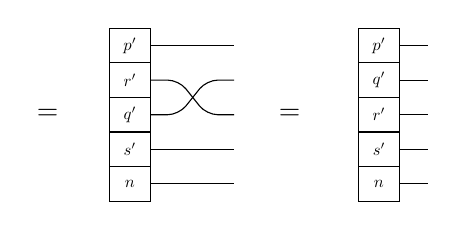
\begin{tikzpicture}[yscale=-1,x=1em,y=1.25em]

    \node[anchor = east] at (0,9){$=$};

    \node[draw, minimum height = 1.25em, minimum width = 1.5em, anchor = east] at (3,7){\scalebox{0.6}{$p'$}};
    \node[draw, minimum height = 1.25em, minimum width = 1.5em, anchor = east] at (3,8){\scalebox{0.6}{$r'$}};
    \node[draw, minimum height = 1.25em, minimum width = 1.5em, anchor = east] at (3,9){\scalebox{0.6}{$q'$}};
    \node[draw, minimum height = 1.25em, minimum width = 1.5em, anchor = east] at (3,10){\scalebox{0.6}{$s'$}};
    \node[draw, minimum height = 1.25em, minimum width = 1.5em, anchor = east] at (3,11){\scalebox{0.6}{$n$}};

    \draw [rounded corners] (3,7) -- (6,7);
    \draw [rounded corners] (3,8) -- (4,8) -- (5,9) -- (6,9);
    \draw [rounded corners] (3,9) -- (4,9) -- (5,8) -- (6,8);
    \draw [rounded corners] (3,10) -- (6,10);
    \draw [rounded corners] (3,11) -- (6,11);

    \node at (8,9) {$=$};

    \node[draw, minimum height = 1.25em, minimum width = 1.5em, anchor = east] at (12,7){\scalebox{0.6}{$p'$}};
    \node[draw, minimum height = 1.25em, minimum width = 1.5em, anchor = east] at (12,8){\scalebox{0.6}{$q'$}};
    \node[draw, minimum height = 1.25em, minimum width = 1.5em, anchor = east] at (12,9){\scalebox{0.6}{$r'$}};
    \node[draw, minimum height = 1.25em, minimum width = 1.5em, anchor = east] at (12,10){\scalebox{0.6}{$s'$}};
    \node[draw, minimum height = 1.25em, minimum width = 1.5em, anchor = east] at (12,11){\scalebox{0.6}{$n$}};


    \draw [rounded corners] (12,7) -- (13,7);
    \draw [rounded corners] (12,8) -- (13,8);
    \draw [rounded corners] (12,9) -- (13,9);
    \draw [rounded corners] (12,10) -- (13,10);
    \draw [rounded corners] (12,11) -- (13,11);

\end{tikzpicture}
\end{document}